%%%%%%%%%%%%%%%%%%%%%%%%%%%%%%%%%%%%%%%%%%%%%%%%%%%%%%%%%%%%%%%%%%%%%%%%%%%%%%%
\chapter{Experimental setup and results}~\label{chap:results}
%%%%%%%%%%%%%%%%%%%%%%%%%%%%%%%%%%%%%%%%%%%%%%%%%%%%%%%%%%%%%%%%%%%%%%%%%%%%%%%

A Linux kernel module was developed incorporating the ideas mentioned in chapters \ref{chap:pds}
and \ref{chap:delta}. The scheduling routines in the Linux kernel (To be specific, \textit{schedule} and \textit{\_\_switch\_to})
were extended using kprobes \cite{kprobes} to add the performance directed scheduling features
The entire system with all the interconnections is shown in figure \ref{fig:entire_seeker}.

The choice to use kprobes \cite{kprobes} a feature essentially used for debugging and instrumentation
from the context of a kernel module pose two possible 
problems. One, kprobes by themselves introduce unnecessary code paths and interrupts causing some
if not significant overhead (Less than 3\%). Secondly, certain functions relating to migration are not exported
to kernel modules and hence indirect and suboptimal procedures were chosen to get the necessary 
functionality. In spite of these disadvantages, having the project as a kernel module accelerated 
the development process. 

For a system with \textit{M} total performance states and \textit{N} total processors, $\Delta$ can 
at most take a value of $N \times (M-1)$. Experiments were carried on a quad-core AMD Opteron (Barcelona),
with mutation intervals ranging from 125ms to 1000ms and delta ranging from 1 through 16. The experiments
were carried out with full logging enabled and all of the six different workloads described in Appendix~\ref{app:benchmark}. 
The logs taken contained information relating to the residency of each processor in each state and was 
translated to average power consumed per processor by correlating it to the numbers mentioned in \cite{AMDPow} and
repeated in Appendix~\ref{app:opteron}. Appendix~\ref{app:mutation_timeline} showcases the system adapting to
each of the various workloads for both the ladder and select schedulers.


\begin{figure}[h!]
  \begin{center}
%    \resizebox{\columnwidth}{!}{
    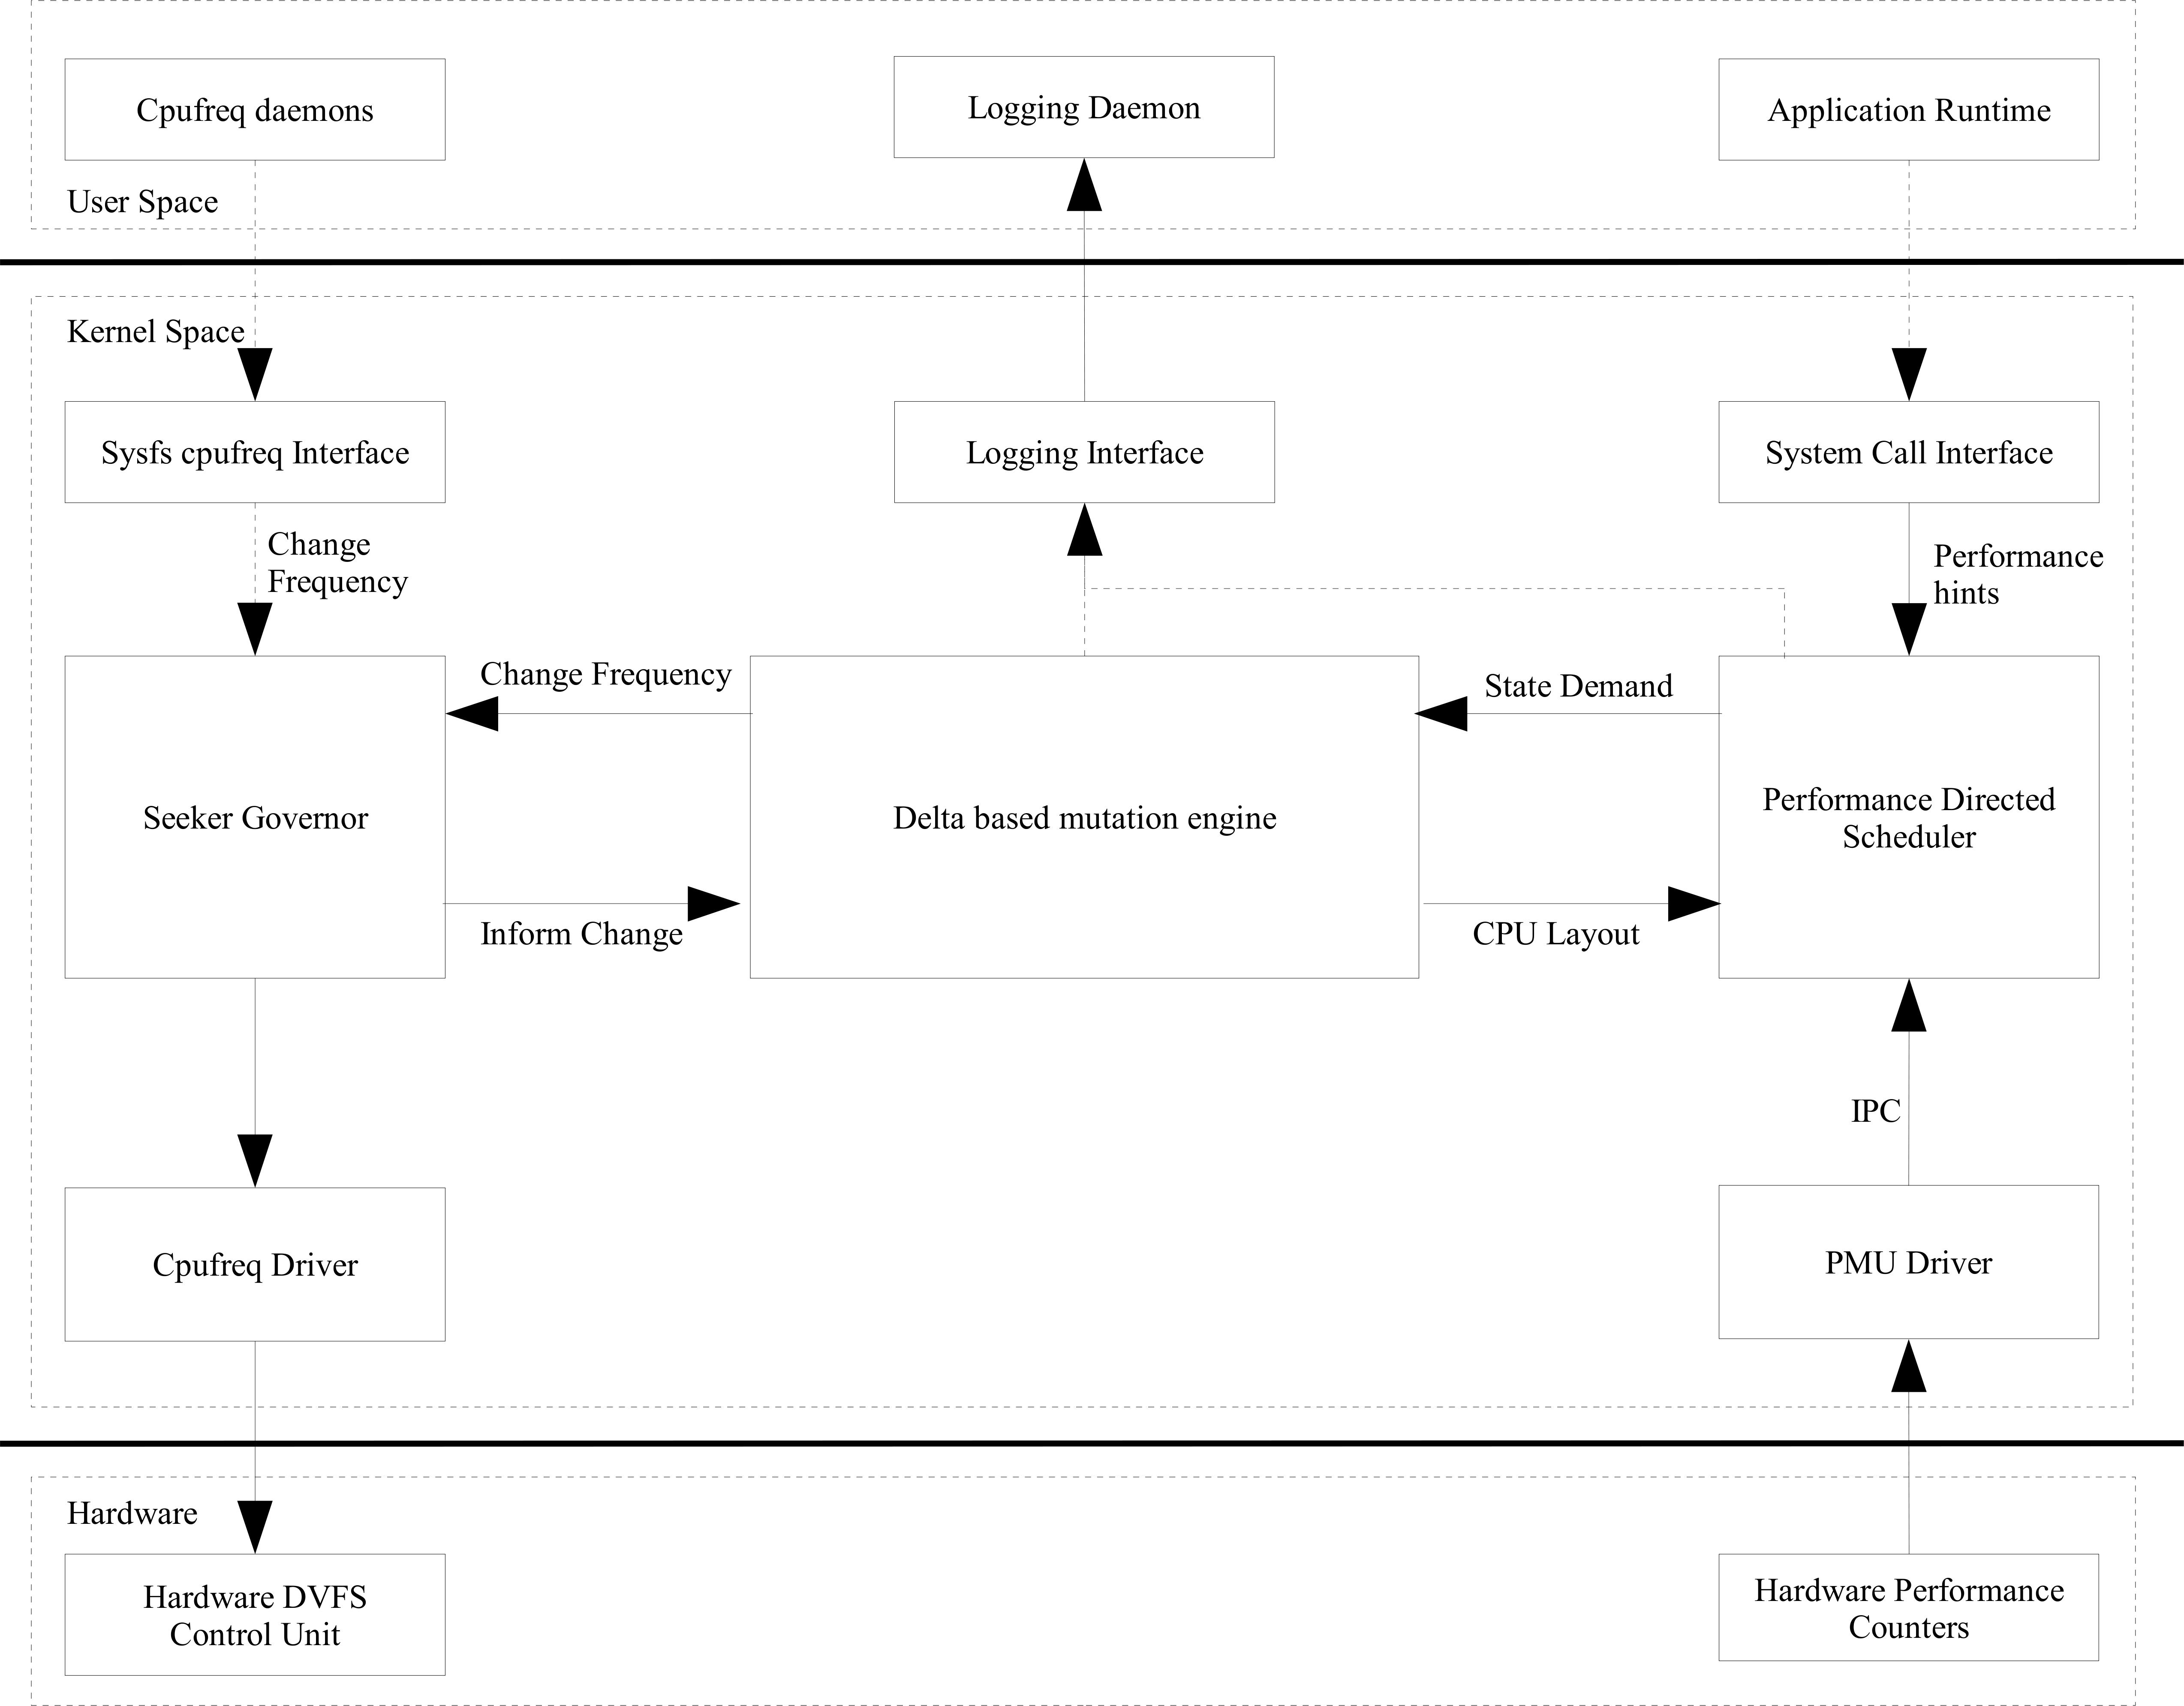
\includegraphics[height=4in]{figures/seeker.jpg}%}
    \caption{The Seeker infrastructure}
    \label{fig:entire_seeker}
  \end{center}
\end{figure}


Three different configurations were run with repeated trials: 
\begin{enumerate}
\item Ondemand governor with scheduling disabled. 
\item Delta mutation engine with the ladder scheduler
\item Delta mutation engine with the select scheduler
\end{enumerate}
The results following which are discussed in further sections. 

%%%%%%%%%%%%%%%%%%%%%%%%%%%%%%%%%%%%%%%%%%%%%%%%%%%%%%%%%%%%%%%%%%%%%%
% START REAL GRAPHS
%%%%%%%%%%%%%%%%%%%%%%%%%%%%%%%%%%%%%%%%%%%%%%%%%%%%%%%%%%%%%%%%%%%%%%
%%%%%%%%%%%%%%%%%%%%%%%%%%%%%%%%%%%%%%%%%%%%%%%%%%%%%%%%%%%%%%%%%%%%%%%%%%%%%%%
\section{Trends along delta and interval}~\label{sec:trends}
%%%%%%%%%%%%%%%%%%%%%%%%%%%%%%%%%%%%%%%%%%%%%%%%%%%%%%%%%%%%%%%%%%%%%%%%%%%%%%%

Two parameters namely the delta constraint ($\Delta$) and the mutation interval 
were introduced in Chapter~\ref{chap:delta}. In order to further study the system
it is important to define the variation of two important effects of the system,
namely, Slowdown and power savings as a function of these parameters. In order
to accomplish this, a fully factorial experiment was conducted varying delta 
from 1 to 16 and the interval from 125ms to 1000ms. All the six workloads in 
Table~\ref{tab:spec_groups} in Appendix~\ref{app:benchmark} were run in each 
experiment.

Figures \ref{fig:slowdown_trends_ladder} and \ref{fig:slowdown_trends_select} show the trends
observed with respect to slowdown for the ladder and select schedulers. An unnaturally 
high slowdown can be observed for small values of delta ($\Delta$). This can easily be attributed
to the plasticity in adaptation. The interval of mutation has little significance towards slowdown
for delta values beyond 3. But as the delta values decrease below 3, the mutation begins to play a vital 
role in differentiating the experiments based on slowdown. It can be observed that at lower values
of delta, reducing the mutation interval has an effect of decreasing the slowdown and effectively 
reducing the performance lost. The differentiating aspect between Figure~\ref{fig:slowdown_trends_ladder} 
and \ref{fig:slowdown_trends_select} is the effect of a low value of delta, at which the select system
provides a very high percentage of slowdown, but both rapidly falls to the plateau close to 16\% beyond 
a delta constraint of 3. 

\begin{figure}[h!]
  \begin{center}
    %\resizebox{\columnwidth}{!}{
    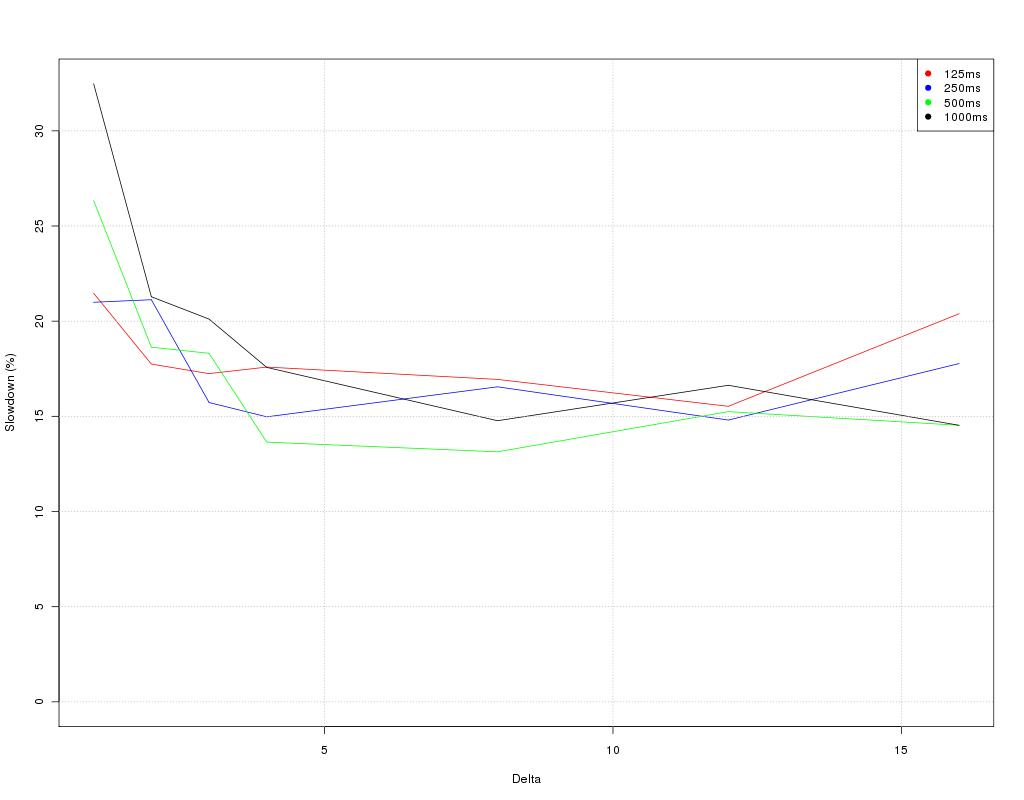
\includegraphics[height=3.5in]{figures/trends_slowdown_ladder.jpg}%}
    \caption{Variation of slowdown with delta and interval with the ladder scheduler}
    \label{fig:slowdown_trends_ladder}
  \end{center}
\end{figure}

\begin{figure}[h!]
  \begin{center}
    %\resizebox{\columnwidth}{!}{
    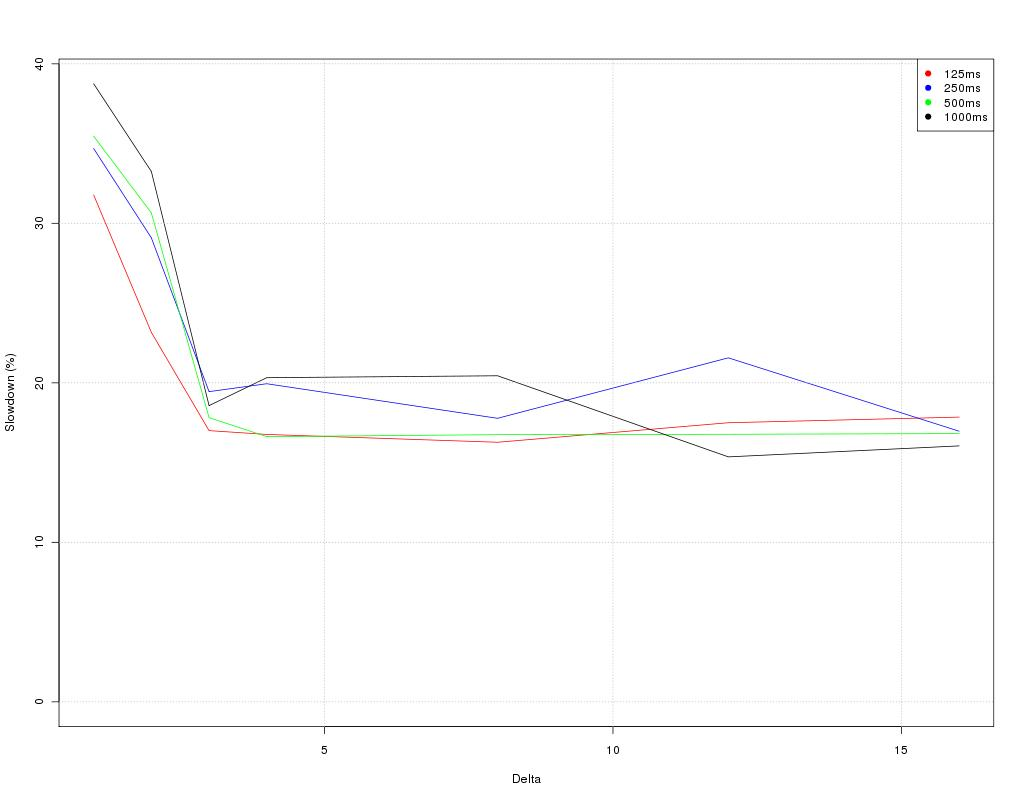
\includegraphics[height=3.5in]{figures/trends_slowdown_select.jpg}%}
    \caption{Variation of slowdown with delta and interval with the select scheduler}
    \label{fig:slowdown_trends_select}
  \end{center}
\end{figure}

Figures \ref{fig:pwr_trends_ladder} and \ref{fig:pwr_trends_select} show the observations 
when the power savings are observed instead of slowdown during the experimentation. 
Even though similar trends to slowdown is observed, one interesting point is that, although
the power savings is quiet high for low values of the delta constraint, it provides 
significant slowdown which is undesirable, but lower values of mutation interval do continue
to provide better power savings. This can clearly be observed for the select scheduler in
Figure~\ref{fig:pwr_trends_select}. Based on these conclusions one can conclude that 
the mutation interval should be as low as possible, but it must be considered that a very
low mutation interval may cause instabilities which are undesirable.

\begin{figure}[h!]
  \begin{center}
    %\resizebox{\columnwidth}{!}{
    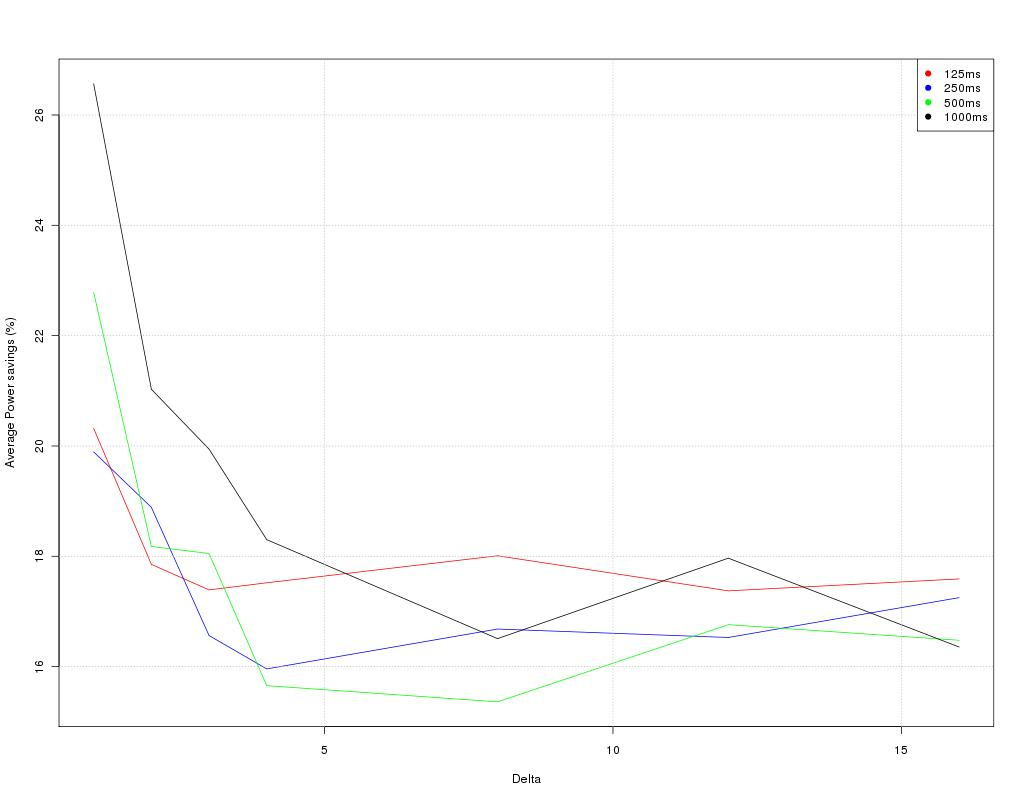
\includegraphics[height=3.5in]{figures/trends_avgpwr_ladder.jpg}%}
    \caption{Variation of power savings with delta and interval with the ladder scheduler}
    \label{fig:pwr_trends_ladder}
  \end{center}
\end{figure}

\begin{figure}[h!]
  \begin{center}
    %\resizebox{\columnwidth}{!}{
    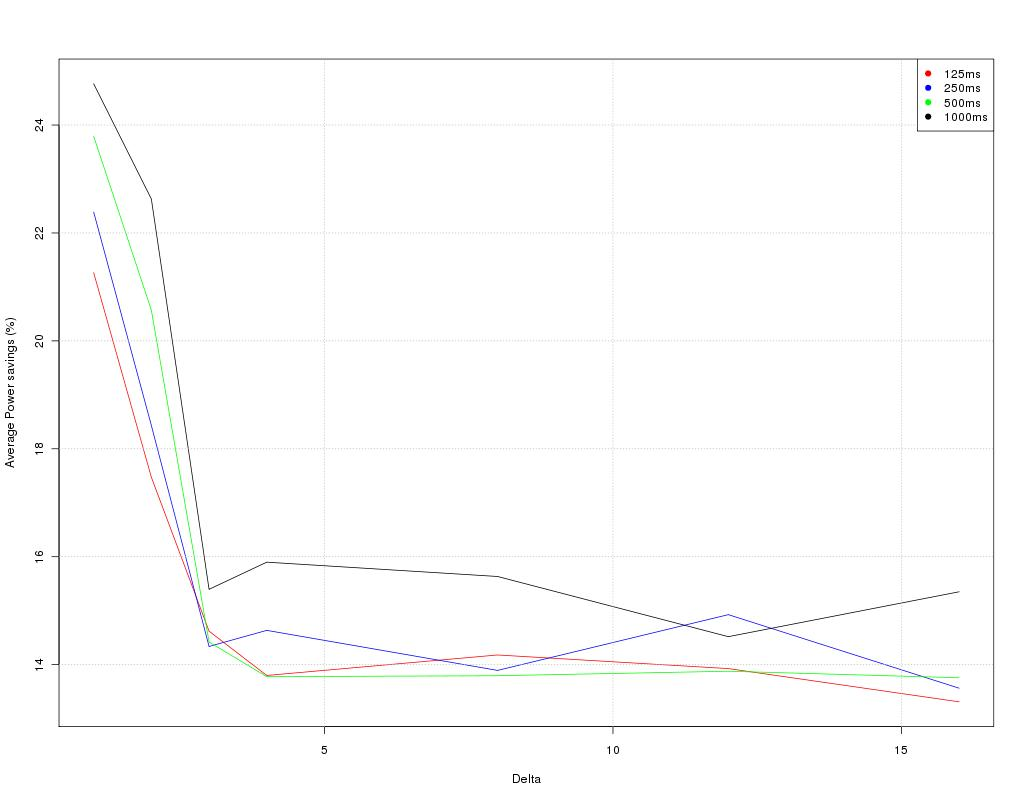
\includegraphics[height=3.5in]{figures/trends_avgpwr_select.jpg}%}
    \caption{Variation of power savings with delta and interval with the select scheduler}
    \label{fig:pwr_trends_select}
  \end{center}
\end{figure}

Based on these observations, it can be concluded that a value of delta $\Delta = 4$ provides
the best among all the compromises and the interval can be changed based on the arrival rate
of jobs on the server or compute node.

%%%%%%%%%%%%%%%%%%%%%%%%%%%%%%%%%%%%%%%%%%%%%%%%%%%%%%%%%%%%%%%%%%%%%%%%%%%%%%%
\section{Effects of workload on power and performance}~\label{sec:wrk_trends}
%%%%%%%%%%%%%%%%%%%%%%%%%%%%%%%%%%%%%%%%%%%%%%%%%%%%%%%%%%%%%%%%%%%%%%%%%%%%%%%

Due to the adaptive nature of the power management mechanism and the high dependence
on the IPC characteristic of the workloads, it can be hypothesized
that workloads with lower IPC (The \textit{Low} workload) should expect the maximum
power savings while, workloads with a large IPC (The \textit{High} workload) should
expect the minimum slowdown and power savings. This is validated from Figures \ref{fig:workload_trends_ladder}
and \ref{fig:workload_trends_select}. The power savings for each workload is plotted
along side the slowdown as a comparison tool. As slowdown is expected, the advantage of the procedure
is the higher power savings than slowdown which both the select and ladder scheduling
procedures exhibit. The \textit{High} workload, suffers insignificant slowdown and 
does not provide with any power savings. The \textit{Low} workload has the greatest advantage
of providing up to 40\% power savings (for the ladder scheduler) with a median of 15\% slowdown.
Similar trends are observed for the select scheduler in Figure~\ref{fig:workload_trends_select} 
except for the lower power savings with the \textit{Low} workload (27\%) for the same amount of 
slowdown.

\begin{figure}[h!]
  \begin{center}
    %\resizebox{\columnwidth}{!}{
    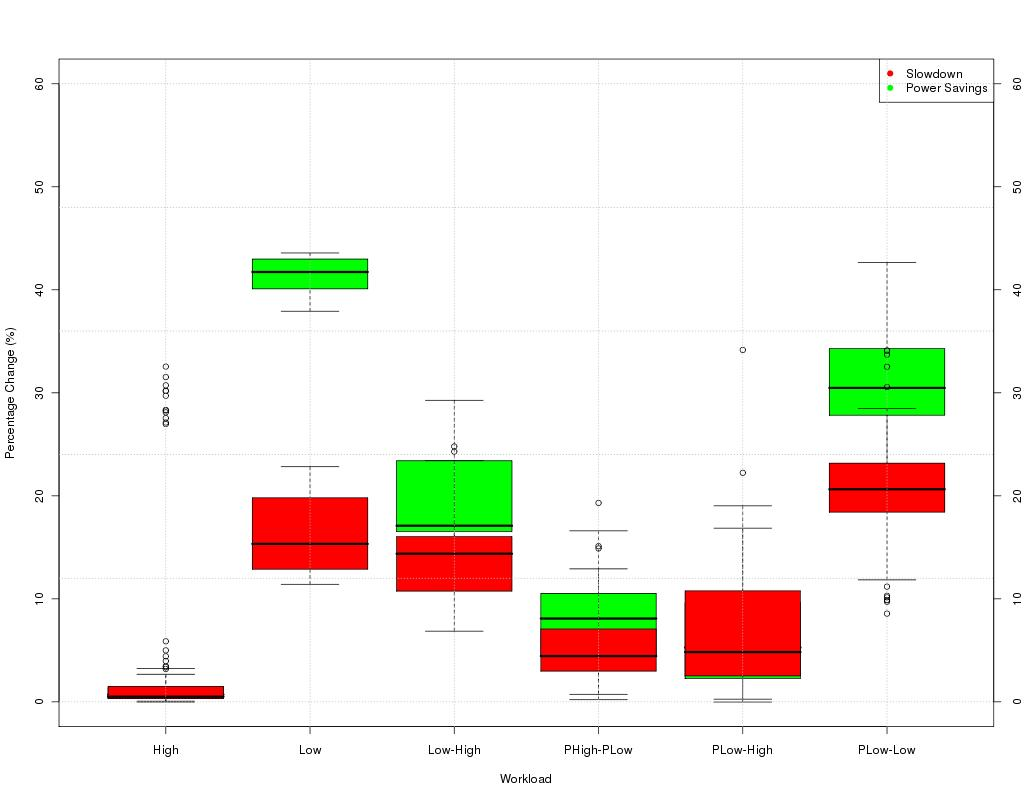
\includegraphics[height=3.5in]{figures/trends_workload_ladder.jpg}%}
    \caption{Variation of slowdown and power savings for each workload with the ladder scheduler}
    \label{fig:workload_trends_ladder}
  \end{center}
\end{figure}

% NEEDS TO BE RE-GENERATED.
\begin{figure}[h!]
  \begin{center}
    %\resizebox{\columnwidth}{!}{
    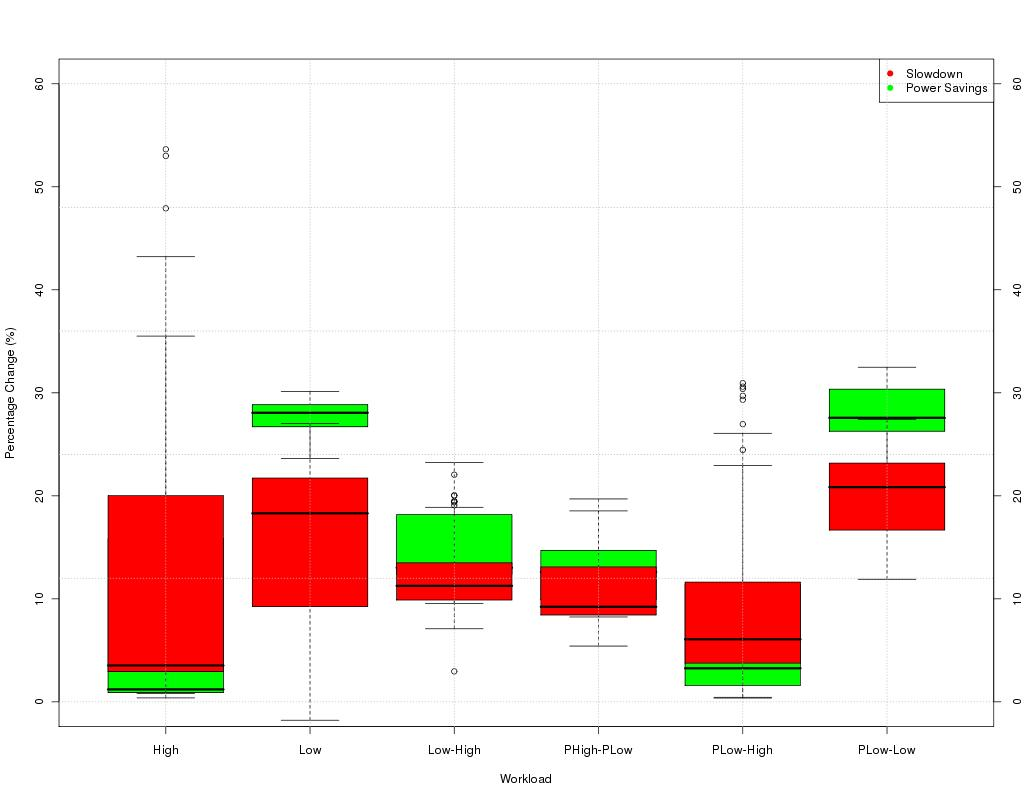
\includegraphics[height=3.5in]{figures/trends_workload_select.jpg}%}
    \caption{Variation of slowdown and power savings for each workload with the select scheduler}
    \label{fig:workload_trends_select}
  \end{center}
\end{figure}

%%%%%%%%%%%%%%%%%%%%%%%%%%%%%%%%%%%%%%%%%%%%%%%%%%%%%%%%%%%%%%%%%%%%%%%%%%%%%%%
\section{Comparing various methodologies}~\label{sec:compare}
%%%%%%%%%%%%%%%%%%%%%%%%%%%%%%%%%%%%%%%%%%%%%%%%%%%%%%%%%%%%%%%%%%%%%%%%%%%%%%%

Chapter~\ref{chap:pds} described two methods of evaluating the performance state and hence
providing two distinct methods of scheduling affecting the adaptation of the delta system.
Hence the two system are separately evaluated in comparison to the \textit{ondemand}
power optimizer. The following three systems were compared in the following experiments:
\begin{itemize}
\item The delta mutator with a delta coefficient of 4 with the ladder scheduler
\item The delta mutator with a delta coefficient of 4 with the select scheduler
\item The ondemand load based governor.
\end{itemize}

As a potential application, these methods may be used with a range of mutation intervals based
on the arrival rate of jobs on the system, the experiments were conducted for varied mutation intervals
in order to demonstrate all possible effects.
Figure~\ref{fig:pwr_vs_slowdown} shows a scatter plot of slowdown plotted against power savings. Each point
represents an experiment/workload which experienced the appropriate slowdown and power savings respectively. 
Points lower indicate a smaller magnitude of slowdown while points farther to the right indicate better power
savings. This graph clearly shows the vice of the Ondemand governor: It does not manage power at active
load and obvious from it's design considerations. This is graphically depicted by all the points pertaining
to the ondemand governor huddled around Power Savings = 0\% and hence providing absolutely no power savings
while the processors are actively executing jobs. The Delta + Select system provides an equal power savings
as the Delta + Ladder except for the workload \textit{Low} for which the ladder system works better in achieving
higher power savings.

% NEEDS TO BE RE-GENERATED.
\begin{figure}[h!]
  \begin{center}
    %\resizebox{\columnwidth}{!}{
    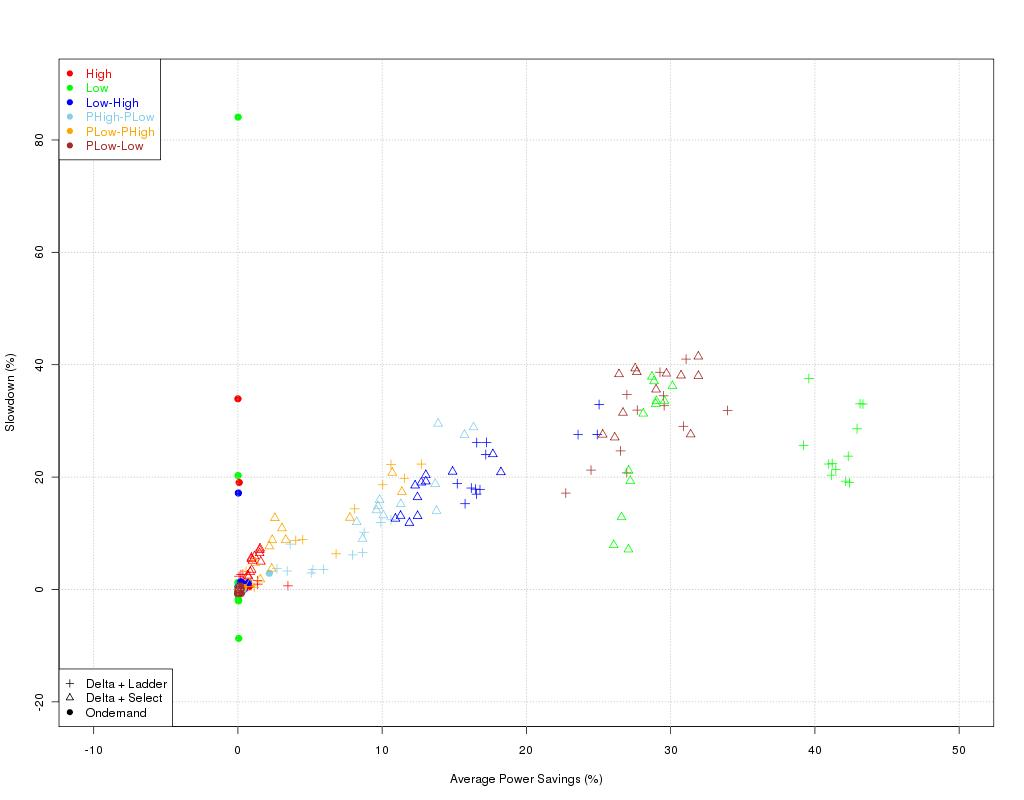
\includegraphics[height=3.5in]{figures/pwr_vs_slowdown_delta_4.jpg}%}
    \caption{Scatter plots showing variation of slowdown with power savings for ondemand, $\Delta=4$ (Select and Ladder)}
    \label{fig:pwr_vs_slowdown}
  \end{center}
\end{figure}

EPI (Energy consumption per instruction) is another important metric which ties in bother throughput and power
consumption. A lower value indicates better energy efficiency. EPI is plotted 
against power savings for each experiment to arrive at Figure~\ref{fig:pwr_vs_jpbi}. As the ondemand governor
does not manage power at execution time, it is observed that not only does it not provide any power savings, 
it ends up utilizing energy inefficiently. Note that the value of EPI for the ondemand governor can be as high
as 170 nW/instruction while both the ladder and select systems exhibit a max EPI of 140 nW/instruction.

% NEEDS TO BE RE-GENERATED.
\begin{figure}[h!]
  \begin{center}
    %\resizebox{\columnwidth}{!}{
    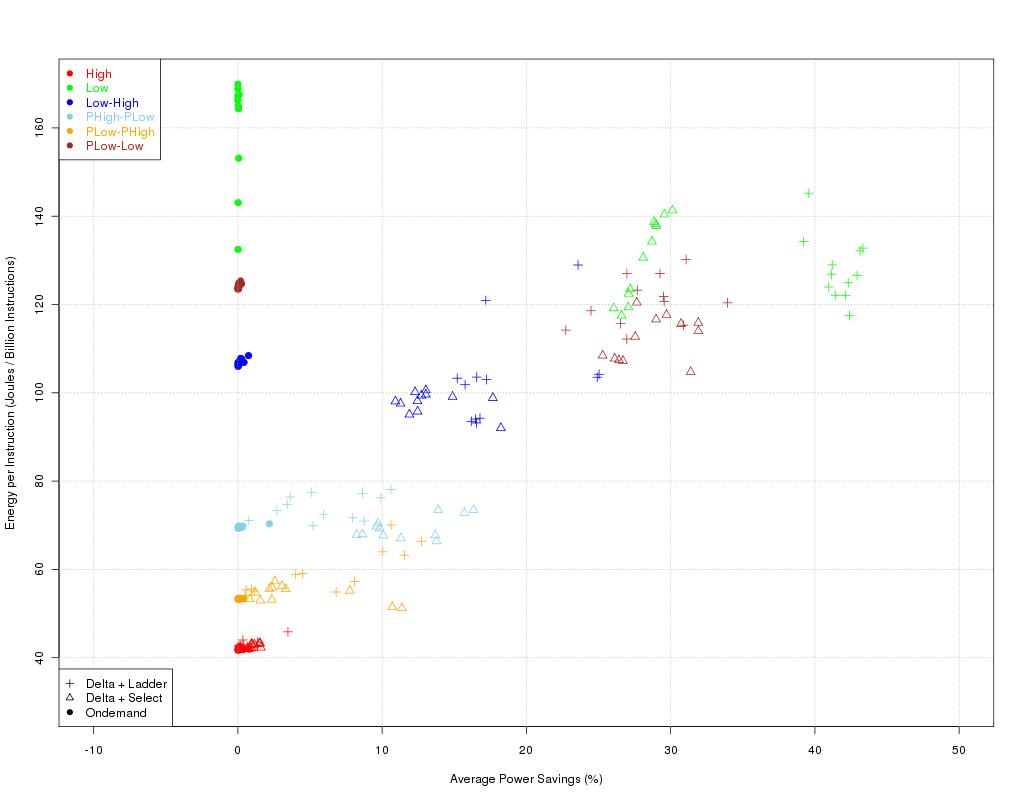
\includegraphics[height=3.5in]{figures/pwr_vs_jpbi_delta_4.jpg}%}
    \caption{Scatter plots showing variation of EPI with power savings for ondemand, $\Delta=4$ (Select and Ladder)}
    \label{fig:pwr_vs_jpbi}
  \end{center}
\end{figure}


An interesting graph \ref{fig:jpbi_vs_slowdown} is arrived at when the scatter plots concentrate on
EPI and slowdown. As we have concluded with figures \ref{fig:pwr_vs_slowdown} and \ref{fig:pwr_vs_jpbi},
the ondemand governor essentially executes all workloads at the highest clock speed (Indicated by 0 slowdown 
and power savings). This allows \ref{fig:jpbi_vs_slowdown} to be viewed to discern if the delta system
does provide a better means to execute workloads in a more energy efficient manner for each workload. This is observable
where all the points pertaining to the delta + select and delta + ladder systems lie to the left of 
the ondemand points for each workload.

% NEEDS TO BE RE-GENERATED.
\begin{figure}[h!]
  \begin{center}
    %\resizebox{\columnwidth}{!}{
    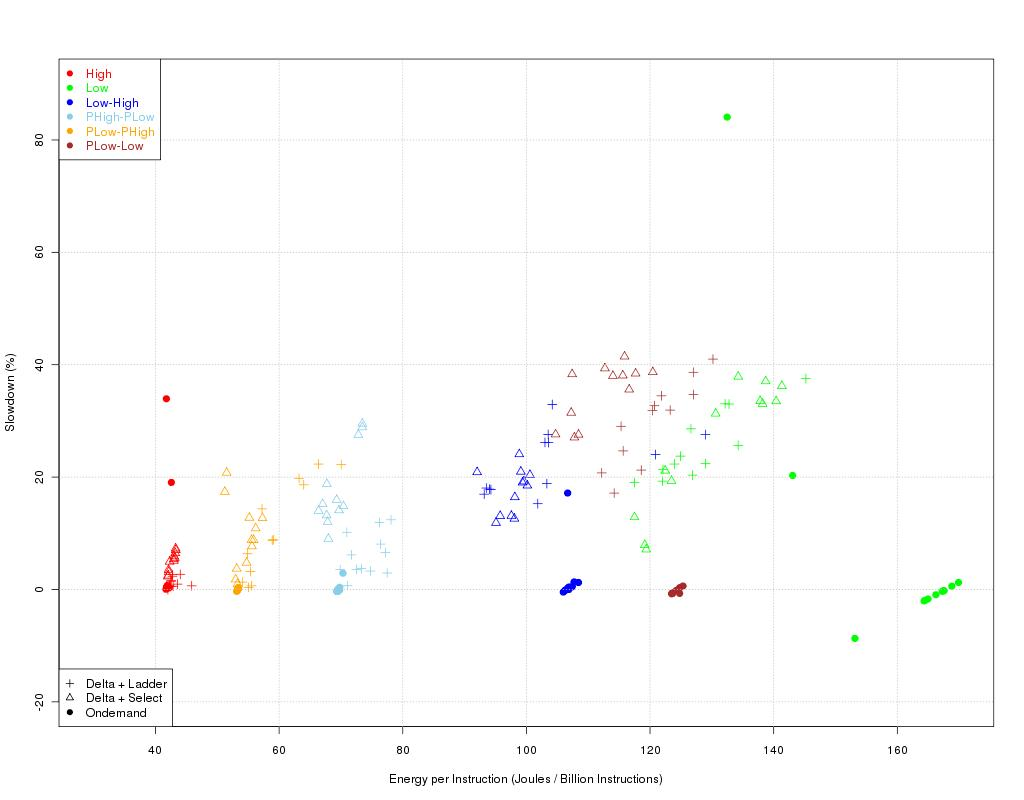
\includegraphics[height=3.5in]{figures/jpbi_vs_slowdown_delta_4.jpg}%}
    \caption{Scatter plots showing variation of slowdown with EPI for ondemand, $\Delta=4$ (Select and Ladder)}
    \label{fig:jpbi_vs_slowdown}
  \end{center}
\end{figure}

%%%%%%%%%%%%%%%%%%%%%%%%%%%%%%%%%%%%%%%%%%%%%%%%%%%%%%%%%%%%%%%%%%%%%%%%%%%%%%%
\section{Power savings and slowdown}~\label{sec:pow_slow}
%%%%%%%%%%%%%%%%%%%%%%%%%%%%%%%%%%%%%%%%%%%%%%%%%%%%%%%%%%%%%%%%%%%%%%%%%%%%%%%

An acceptable power management system demands the relation between power savings and slowdown to be linear
(A slope of 1 at best). Figure~\ref{fig:slowdown_power_ladder} shows a very pleasing slope of 1 indicating 
equal power savings for every percent of slowdown. But even though the select scheduler is better by hypothesis, 
it ends up giving closer to 8\% power savings for every 10\% slowdown (Figure~\ref{fig:slowdown_power_select}). 


\begin{figure}[h!]
  \begin{center}
    %\resizebox{\columnwidth}{!}{
    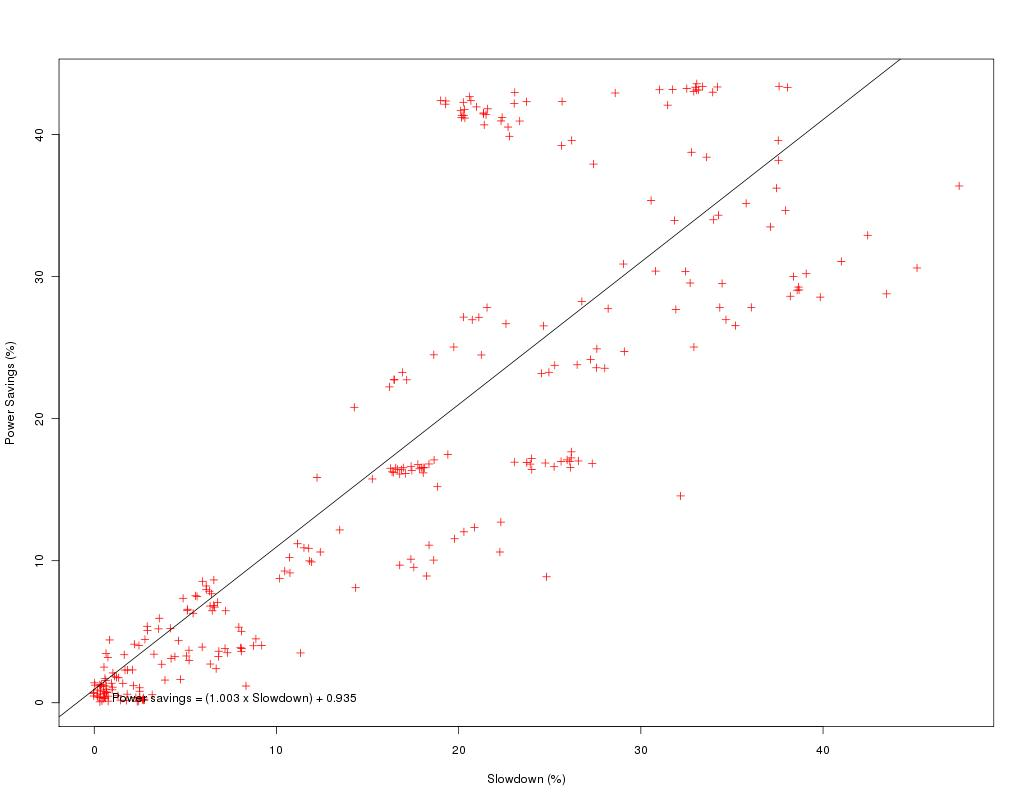
\includegraphics[height=3.5in]{figures/slowdown_power_ladder.jpg}%}
    \caption{Trends over workload variation}
    \label{fig:slowdown_power_ladder}
  \end{center}
\end{figure}

% NEEDS TO BE RE-GENERATED.
\begin{figure}[h!]
  \begin{center}
    %\resizebox{\columnwidth}{!}{
    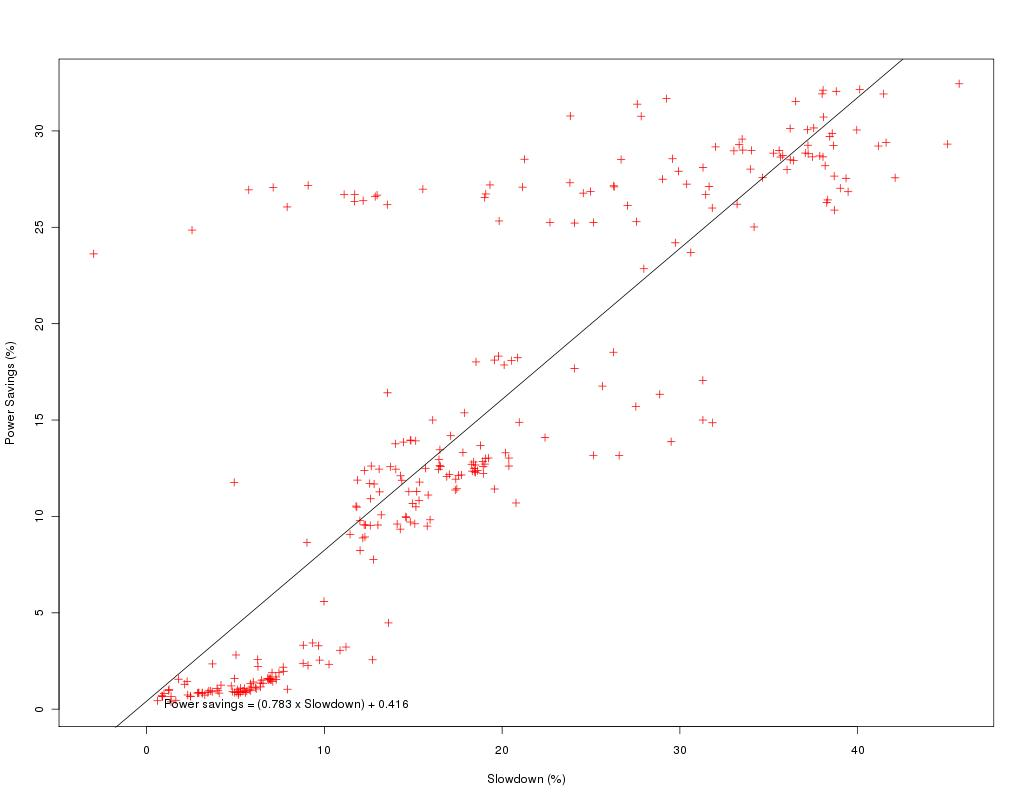
\includegraphics[height=3.5in]{figures/slowdown_power_select.jpg}%}
    \caption{Trends over workload variation}
    \label{fig:slowdown_power_select}
  \end{center}
\end{figure}

%%%%%%%%%%%%%%%%%%%%%%%%%%%%%%
% Do I need to write more? 
%%%%%%%%%%%%%%%%%%%%%%%%%%%%%%
